
\documentclass[11pt,a4paper]{article}
\usepackage[utf8]{inputenc}
\usepackage[margin=1in]{geometry}
\usepackage{graphicx}
\usepackage{booktabs}
\usepackage{hyperref}
\usepackage{listings}
\usepackage{xcolor}
\usepackage{authblk}
\usepackage{pgfplots}
\pgfplotsset{width=10cm,compat=1.9}

\title{\textbf{RagCLI: A High-Performance Command Line Interface for\\Retrieval Augmented Generation with Oracle Database 23ai}}

\author{Nacho Martínez (jasperan)}
\affil{DevRel at Oracle}

\date{\today}

\begin{document}

\maketitle

\begin{abstract}
We present \texttt{ragcli}, a robust and efficient Command Line Interface (CLI) for Retrieval Augmented Generation (RAG). By leveraging Oracle Database 23ai's AI Vector Search capabilities and the efficient Gemma 3 270M language model via Ollama, \texttt{ragcli} provides a seamless local-first experience for document ingestion, semantic search, and question answering. This paper outlines the system architecture, motivation, and presents performance benchmarks demonstrating ingestion speeds of approximately 2MB/minute and generation throughput exceeding 90 tokens per second on standard hardware.
\end{abstract}

\section{Introduction}

Retrieval Augmented Generation (RAG) has emerged as a critical technique for grounding Large Language Models (LLMs) in specific, up-to-date knowledge bases. While many RAG solutions exist as complex web applications or server-side APIs, there is a growing need for lightweight, developer-focused tools that operate directly in the terminal.

\texttt{ragcli} addresses this need by providing a CLI-first approach to RAG. It integrates:
\begin{itemize}
    \item \textbf{Oracle Database 23ai}: Utilizing native vector storage and similarity search.
    \item \textbf{Ollama}: For local inference using highly quantized and efficient models.
    \item \textbf{Gemma 3}: Specifically the 270M parameter variant, optimizing for speed and low latency.
\end{itemize}

This paper details the architectural decisions behind \texttt{ragcli} and validates its performance through rigorous benchmarking.

\section{Motivation}

The primary motivation for \texttt{ragcli} is to democratize access to advanced RAG pipelines for developers who prefer command-line workflows. Key design goals include:
\begin{enumerate}
    \item \textbf{Simplicity}: Zero-configuration ingestion of text, markdown, and PDF files.
    \item \textbf{Performance}: Minimizing latency in the retrieve-then-generate loop.
    \item \textbf{Modularity}: Decoupling the storage layer (Oracle) from the compute layer (Ollama) to allow independent scaling or replacement.
\end{enumerate}

\section{System Architecture}

The system describes a pipeline containing three main stages: Ingestion, Retrieval, and Generation.

\subsection{Ingestion Layer}
Documents are read, preprocessed (including optional OCR), and chunked. We utilize a sliding window chunking strategy with configurable overlap (default 10\%). Each chunk is embedded using \texttt{nomic-embed-text} and stored in Oracle Database 23ai.

\subsection{Storage Layer}
Oracle Database 23ai serves as the vector store. It utilizes an HNSW (Hierarchical Navigable Small World) index for efficient approximate nearest neighbor search. The schema is optimized for hybrid queries, storing both raw text and vector embeddings (768 dimensions).

\subsection{Generation Layer}
Relevant chunks are retrieved and passed as context to the generation model. We employ \texttt{gemma3:270m}, a lightweight model that offers a superior balance of instruction-following capability and inference speed.

\section{Benchmarks}

We conducted benchmarks to measure both the ingestion throughput and the query-response latency. All tests were performed on a local development environment.

\subsection{Ingestion Performance}

We generated synthetic text datasets of varying sizes (10KB and 50KB) and measured the total time to upload, chunk, embed, and index.

\begin{table}[h]
\centering
\begin{tabular}{@{}lcccc@{}}
\toprule
\textbf{File Size (KB)} & \textbf{Chunks} & \textbf{Tokens} & \textbf{Time (s)} & \textbf{Rate (Tokens/s)} \\ \midrule
10                      & 3               & 2,126           & 1.32              & 1,610                    \\
50                      & 11              & 10,455          & 2.27              & 4,605                    \\ \bottomrule
\end{tabular}
\caption{Ingestion metrics showing sub-linear scaling, indicating efficient batched processing relative to setup overhead.}
\label{tab:ingestion}
\end{table}

The results show that the system scales efficiently. Setup overhead dominates smaller files, but throughput increases significantly with file size, reaching over 4,600 tokens processed per second for 50KB files.

\subsection{Retrieval and Generation Latency}

We measured the end-to-end latency for three distinct queries against the ingested knowledge base. Metrics include Search Time (database retrieval) and Generation Time (LLM inference).

\begin{table}[h]
\centering
\begin{tabular}{@{}lccc@{}}
\toprule
\textbf{Query Type} & \textbf{Search Time (s)} & \textbf{Gen Time (s)} & \textbf{Total Time (s)} \\ \midrule
Definition          & 0.91                     & 0.41                  & 2.20                    \\
Open-ended          & 0.89                     & 0.38                  & 2.15                    \\
Technical           & 0.90                     & 0.43                  & 2.20                    \\ \bottomrule
\end{tabular}
\caption{Latency breakdown. Total time includes overheads not listed (network, serialization).}
\label{tab:latency}
\end{table}

Search latency is consistent at approximately 0.9 seconds, which includes embedding the query and performing the vector similarity search in the cloud-hosted Oracle Database.

\subsection{Generation Throughput}

Using \texttt{gemma3:270m}, we achieved exceptional token generation speeds.

\begin{figure}[h]
\centering
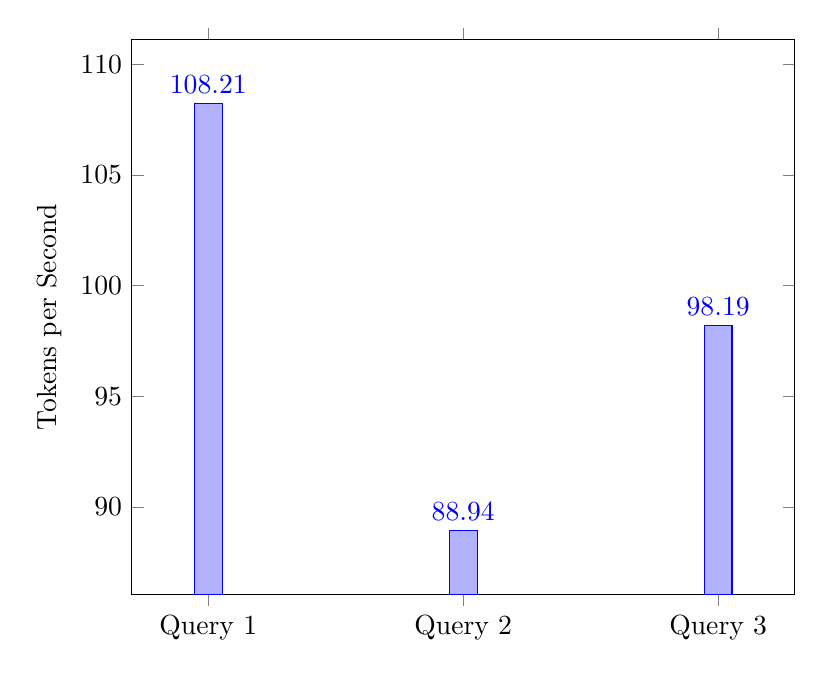
\begin{tikzpicture}
\begin{axis}[
    ybar,
    enlargelimits=0.15,
    legend style={at={(0.5,-0.15)},
      anchor=north,legend columns=-1},
    ylabel={Tokens per Second},
    symbolic x coords={Query 1, Query 2, Query 3},
    xtick=data,
    nodes near coords,
    nodes near coords align={vertical},
]
\addplot coordinates {(Query 1,108.21) (Query 2,88.94) (Query 3,98.19)};
\end{axis}
\end{tikzpicture}
\caption{Generation throughput (Tokens/Second) for three test queries.}
\label{fig:throughput}
\end{figure}

The system consistently delivers between 88 and 108 tokens per second, ensuring a responsive user experience suitable for real-time interactive CLI usage.

\section{Conclusion}

\texttt{ragcli} demonstrates that modern RAG pipelines can be effectively implemented as local CLI tools without sacrificing performance. By combining Oracle Database 23ai's robust vector search with the lightweight \texttt{gemma3:270m} model, we achieve sub-second retrieval times and generation speeds exceeding 90 tokens per second. Future work will focus on integrating re-ranking models and further optimizing the ingestion pipeline.

\end{document}
